\studynote{3}{Wed 12 Oct 2022 18:36}{Autocorrelation Function}

The reference used is \cite{brockwellIntroductionTimeSeries2016}. Essential definitions are given below.

\begin{definition}(Mean and Covariance)
Let $\left\{X_t\right\}$ be a time series with $E\left(X_t^2\right)<\infty$. The mean function of $\left\{X_t\right\}$ is
\[
\mu_X(t)=E\left(X_t\right) .
\]
The covariance function of $\left\{X_t\right\}$ is
\[
\gamma_X(r, s)=\operatorname{Cov}\left(X_r, X_s\right)=E\left[\left(X_r-\mu_X(r)\right)\left(X_s-\mu_X(s)\right)\right]
\]
for all integers $r$ and $s$.
\end{definition}

\begin{definition}[Stationary Time Series]
	$\left\{X_t\right\}$ is (weakly) stationary if
(i) $\mu_X(t)$ is independent of $t$, and
(ii) $\gamma_X(t+h, t)$ is independent of $t$ for each $h$.
\end{definition}

\begin{definition}[Autocorrelation Function]
	Let $\left\{X_t\right\}$ be a stationary time series. The autocovariance function (ACVF) of $\left\{X_t\right\}$ at lag $h$ is
\[
\gamma_X(h)=\operatorname{Cov}\left(X_{t+h}, X_t\right) .
\]
The autocorrelation function (ACF) of $\left\{X_t\right\}$ at lag $h$ is
\[
\rho_X(h) \equiv \frac{\gamma_X(h)}{\gamma_X(0)}=\operatorname{Cor}\left(X_{t+h}, X_t\right)
\]
\end{definition}


\begin{example}
	\begin{enumerate}
		\item (i.i.d. noise) If $\left\{X_t\right\}$ is iid noise and $E\left(X_t^2\right)=\sigma^2<\infty$,we have
\[
	\gamma_X(t+h, t)= \begin{cases}\sigma^2, & \text { if } h=0 \\ 0, & \text { if } h \neq 0\end{cases}
.\] 
Thus
\[
	\rho_X(h) = \begin{cases}
		1 & h = 0\\
		0 & h \neq  0
	\end{cases}
.\] 
\begin{figure}[h]
	\centering
	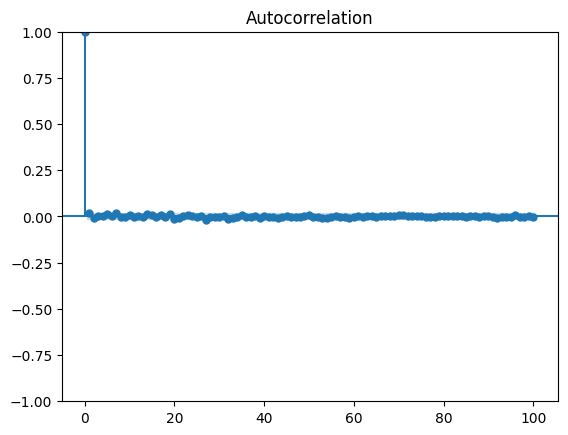
\includegraphics[width=0.6\textwidth]{figures/iid_noise_acf.png}
	\caption{Example of a calculated ACF for i.i.d process}
	\label{fig:figures-iid_noise_acf-png}
\end{figure}
\item (First-Order Moving Average or MA(1) Process)
Consider the series defined by the equation
\[
X_t=Z_t+\theta Z_{t-1}, \quad t=0, \pm 1, \ldots,
\]
where $\left\{Z_t\right\} \sim \mathrm{WN}\left(0, \sigma^2\right)$ and $\theta$ is a real-valued constant. From above we see that $E X_t=0, E X_t^2=\sigma^2\left(1+\theta^2\right)<\infty$, and
\[
\gamma_X(t+h, t)= \begin{cases}\sigma^2\left(1+\theta^2\right), & \text { if } h=0 \\ \sigma^2 \theta, & \text { if } h=\pm 1 \\ 0, & \text { if }|h|>1\end{cases}
\]
Thus $\left\{X_t\right\}$ is stationary. The autocorrelation function of $\left\{X_t\right\}$ is
\[
\rho_X(h)= \begin{cases}1, & \text { if } h=0 \\ \theta /\left(1+\theta^2\right), & \text { if } h=\pm 1 \\ 0, & \text { if }|h|>1\end{cases}
\]
	\end{enumerate}
\end{example}

\begin{definition}[Strictly Stationary](2.1.2)
	$\left\{X_t\right\}$ is a strictly stationary time series if
\[
\left(X_1, \ldots, X_n\right)^{\prime} \stackrel{d}{=}\left(X_{1+h}, \ldots, X_{n+h}\right)^{\prime}
\]
for all integers $h$ and $n \geq 1$. (Here $\stackrel{d}{=}$ is used to indicate that the two random vectors have the same joint distribution function.)
\end{definition}

\begin{proposition}
	Properties of a Strictly Stationary Time Series $\left\{X_t\right\}$ :\\
a. The random variables $X_t$ are identically distributed.\\
b. $\left(X_t, X_{t+h}\right)^{\prime} \stackrel{d}{=}\left(X_1, X_{1+h}\right)^{\prime}$ for all integers $t$ and $h$.\\
c. $\left\{X_t\right\}$ is weakly stationary if $E\left(X_t^2\right)<\infty$ for all $t$.\\
d. Weak stationarity does not imply strict stationarity.\\
e. An iid sequence is strictly stationary.
\end{proposition}
